% Figure: the cascade over a knot ladder, and one Matern stage as forward and backward
% first-order sections. Referenced from section 7. Pure TikZ, schematic (2026-09-18, the
% author's review). Top: the knot ladder, exact at every knot (prop:knot-exactness). Bottom:
% one stage for integer gamma (prop:matern-cascade).

\begin{figure}[t]
\centering
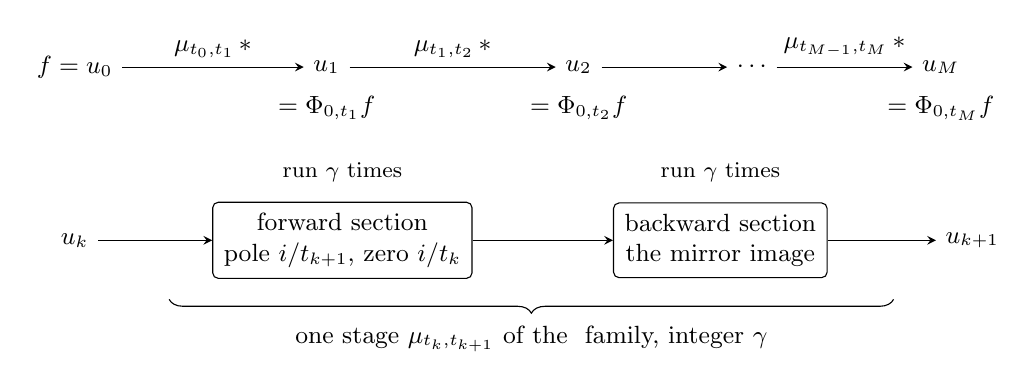
\begin{tikzpicture}[every node/.style={font=\small}, >=stealth,
  box/.style={draw, rounded corners=2pt, minimum height=8mm, inner sep=4pt, align=center}]

% --- the knot ladder ------------------------------------------------------------------------
\node (u0) at (0,2.2) {$f = u_0$};
\node (u1) at (3.2,2.2) {$u_1$};
\node (u2) at (6.4,2.2) {$u_2$};
\node (ud) at (8.6,2.2) {$\cdots$};
\node (uM) at (11.0,2.2) {$u_M$};
\draw[->] (u0) -- node[above] {$\mu_{t_0,t_1}\,*$} (u1);
\draw[->] (u1) -- node[above] {$\mu_{t_1,t_2}\,*$} (u2);
\draw[->] (u2) -- (ud);
\draw[->] (ud) -- node[above] {$\mu_{t_{M-1},t_M}\,*$} (uM);
\node[anchor=north] at (3.2,1.95) {$= \Phi_{0,t_1}f$};
\node[anchor=north] at (6.4,1.95) {$= \Phi_{0,t_2}f$};
\node[anchor=north] at (11.0,1.95) {$= \Phi_{0,t_M}f$};

% --- one Matern stage -----------------------------------------------------------------------
\node (in) at (0,0) {$u_k$};
\node[box] (fw) at (3.4,0) {forward section\\ pole $i/t_{k+1}$, zero $i/t_k$};
\node[box] (bw) at (8.2,0) {backward section\\ the mirror image};
\node (out) at (11.4,0) {$u_{k+1}$};
\draw[->] (in) -- (fw);
\draw[->] (fw) -- (bw);
\draw[->] (bw) -- (out);
\node[anchor=south] at (3.4,0.62) {\footnotesize run $\gamma$ times};
\node[anchor=south] at (8.2,0.62) {\footnotesize run $\gamma$ times};
\draw[decorate, decoration={brace, amplitude=5pt, mirror}] (1.2,-0.75) -- (10.4,-0.75)
  node[midway, below=6pt] {one stage $\mu_{t_k,t_{k+1}}$ of the \Matern{} family, integer $\gamma$};

\end{tikzpicture}
\caption{The cascade as an algorithm. Top: over any ladder of scale knots the cascade of
stages reproduces the scale space exactly at every knot
(Proposition~\ref{prop:knot-exactness}). Bottom: for the \Matern{} family with integer
$\gamma$, a stage is $\gamma$ first-order recursive sections run forward along the signal
followed by $\gamma$ run backward (the label above a box says how often its section is run), each with
one state and with positive coefficients
(Proposition~\ref{prop:matern-cascade}).}
\label{fig:sections}
\end{figure}
